% ======================================================================
%  Chapter 12 — Valleys and Lattices  (EXPANDED)
% ======================================================================

\section{Inversion breaking as an alternative}
\label{sec:ch12-inversion-breaking}

In \chref{ch:breaking-tr} we saw that breaking time-reversal symmetry
at a pair of Dirac cones produces bands with nonzero Chern numbers,
because the Berry-flux contributions from $K$ and $K'$ \emph{add}.
There is another route to lifting the Dirac degeneracy: breaking
\emph{inversion} symmetry while preserving time reversal.  In this case
the Berry fluxes at $K$ and $K'$ have \emph{opposite} signs and the
global Chern number vanishes, but the \emph{valley-resolved} Berry flux
is nonzero and can support edge modes at domain walls between regions
with opposite inversion breaking
\cite{kang2018pseudo}.

This ``valley-Hall'' mechanism has become one of the most widely used
approaches to topological photonics
\cite{ma2016all,dong2016valley,ozawa2018topological}, because it requires neither
magneto-optical materials nor time modulation---only a geometric
asymmetry in the unit cell.

\section{Symmetry analysis of inversion breaking}
\label{sec:ch12-symmetry}

\subsection{Inversion in a honeycomb lattice}
\label{sec:ch12-inversion-honeycomb}

A honeycomb photonic crystal (e.g.\ a hexagonal arrangement of two
sublattices $A$ and $B$) has $C_{6v}$ symmetry when the two sublattices
are identical.  The inversion operation $\Pop$ exchanges $A$ and $B$
while reversing $\rvec\to-\rvec$.

When the sublattices are made inequivalent (different rod radii, hole
sizes, or material compositions), the $C_{6v}$ symmetry is reduced to
$C_{3v}$: the threefold rotation $C_3$ and the three mirror planes
$\sigma_v$ are preserved, but inversion $\Pop$ and the remaining
mirrors are broken.

\subsection{Effect on Dirac points}
\label{sec:ch12-effect-dirac}

Recall from \secref{sec:ch6-real-symmetric} that Dirac points in a
hexagonal lattice are protected by the combination of $\Top$ and $\Pop$.
Under the von Neumann--Wigner codimension argument:
\begin{itemize}
  \item With $\Top+\Pop$: the eigenproblem is real symmetric, requiring
  only 2 conditions for degeneracy in a 2D parameter space---generically
  allowed.
  \item With $\Top$ alone (no $\Pop$): the eigenproblem is complex
  Hermitian, requiring 3 conditions---generically forbidden in 2D.
\end{itemize}
Thus, breaking $\Pop$ while preserving $\Top$ lifts the Dirac
degeneracy generically.

\subsection{The mass term from sublattice asymmetry}
\label{sec:ch12-mass-derivation}

To derive the mass term explicitly, we return to the two-mode effective
equation at the Dirac point (\secref{sec:ch6-two-mode}).  Let the
unperturbed crystal have $C_{6v}$ symmetry with Dirac modes
$|\mathbf{u}_\pm(\kvec_K)\rangle$ transforming under the
two-dimensional irreducible representation $E_1$ of $C_{3v}$.

The sublattice asymmetry is described by a perturbation
$\delta\Mmat(\rvec)$ that is invariant under $C_3$ but odd under $\Pop$
(it has opposite signs on the two sublattices).  In the two-mode
subspace, the perturbation matrix has the form:
\begin{equation}\label{eq:ch12-perturbation-matrix}
  \delta H = \begin{pmatrix}
    \langle\mathbf{u}_+|\delta\Mmat|\mathbf{u}_+\rangle &
    \langle\mathbf{u}_+|\delta\Mmat|\mathbf{u}_-\rangle \\
    \langle\mathbf{u}_-|\delta\Mmat|\mathbf{u}_+\rangle &
    \langle\mathbf{u}_-|\delta\Mmat|\mathbf{u}_-\rangle
  \end{pmatrix}.
\end{equation}

By the symmetry of $C_3$: if the modes $|\mathbf{u}_\pm\rangle$ are
chosen to transform as $\ee^{\pm\ii 2\pi/3}$ under $C_3$, then the
off-diagonal elements vanish (they would require $\delta\Mmat$ to
transform nontrivially under $C_3$, but the sublattice perturbation is
$C_3$-invariant).  The diagonal elements are equal and opposite:
$\langle\mathbf{u}_+|\delta\Mmat|\mathbf{u}_+\rangle
=-\langle\mathbf{u}_-|\delta\Mmat|\mathbf{u}_-\rangle\equiv m_\Delta$,
because $\Pop$ exchanges $|\mathbf{u}_+\rangle$ and
$|\mathbf{u}_-\rangle$ while reversing the sign of $\delta\Mmat$.

Thus the perturbation is proportional to $\sigma_z$:
\begin{equation}\label{eq:ch12-mass-sigma-z}
  \delta H = m_\Delta\,\sigma_z\,,
  \qquad m_\Delta \propto \Delta\,,
\end{equation}
where $\Delta$ parametrises the sublattice asymmetry (e.g.\ $\Delta=
r_A-r_B$ for rod radii).  The full effective Hamiltonian near $K$ is the
massive Dirac equation:
\begin{equation}\label{eq:ch12-massive-dirac-K}
  H_K(\delta\kvec) = v_D(\delta k_x\sigma_x+\delta k_y\sigma_y)
  + m_\Delta\sigma_z\,.
\end{equation}

\subsection{Opposite masses at K and K-prime}
\label{sec:ch12-opposite-masses}

The crucial difference from the gyrotropic case
(\chref{ch:breaking-tr}) is the behaviour under time reversal.  Time
reversal maps $K\to K'$ and complex-conjugates the Hamiltonian.  Since
$m_\Delta$ is real and time-reversal even, but the Dirac matrices at
$K'$ are related to those at $K$ by complex conjugation:
\begin{equation}\label{eq:ch12-massive-dirac-Kprime}
  H_{K'}(\delta\kvec) = v_D(-\delta k_x\sigma_x+\delta k_y\sigma_y)
  - m_\Delta\sigma_z\,.
\end{equation}
The mass at $K'$ is $-m_\Delta$: \emph{opposite} to the mass at $K$.
This can also be seen from the constraint $\Omega_n(\kvec)
=-\Omega_n(-\kvec)$ imposed by time-reversal symmetry: the Berry
curvature must be odd under $\kvec\to-\kvec$, forcing opposite signs
at the two valleys.

\section{Valley Chern numbers}
\label{sec:ch12-valley-chern}

\subsection{Definition and half-integer quantisation}
\label{sec:ch12-valley-def}

The Berry curvature near each valley has the massive Dirac form
(\eqnref{eq:ch7-bc-result}):
\begin{equation}\label{eq:ch12-valley-curvature}
  \Omega_n(\kvec)\Big|_{\text{near }K}
  = +\frac{m_\Delta}{2\bigl(|\delta\kvec|^2+m_\Delta^2\bigr)^{3/2}}\,,
  \quad
  \Omega_n(\kvec)\Big|_{\text{near }K'}
  = -\frac{m_\Delta}{2\bigl(|\delta\kvec|^2+m_\Delta^2\bigr)^{3/2}}\,.
\end{equation}
The total Chern number $\Chern_n=(2\pi)^{-1}\int_\BZ\Omega_n\,\dd^2k=0$
vanishes as required by time-reversal symmetry.

The \emph{valley Chern number} integrates the Berry curvature over only
half of the Brillouin zone surrounding each valley
\cite{dong2016valley,noh2017observation}:
\begin{equation}\label{eq:ch12-valley-chern}
  \Chern_n^K = \frac{1}{2\pi}\int_{\text{near }K}\Omega_n\,\dd^2k
  = +\frac{1}{2}\sgn(m_\Delta)\,,
  \qquad
  \Chern_n^{K'} = -\frac{1}{2}\sgn(m_\Delta)\,.
\end{equation}

\begin{remark}
The valley Chern number is \emph{not} a true topological invariant---it
depends on how the Brillouin zone is partitioned into two halves.
However, when the Berry curvature is sharply localised near the Dirac
points (small gap relative to bandwidth), the partition ambiguity is
exponentially small.  The valley Chern number becomes a useful
approximate invariant in this regime.
\end{remark}

\subsection{The valley-contrast Chern number}
\label{sec:ch12-valley-contrast}

The difference between the two valley Chern numbers:
\begin{equation}\label{eq:ch12-Cv}
  \Chern_v = \Chern_n^K - \Chern_n^{K'} = 2\Chern_n^K
  = \sgn(m_\Delta) = \pm 1\,.
\end{equation}
At a domain wall between two regions with opposite sublattice asymmetry
($\Delta>0$ on one side, $\Delta<0$ on the other), the valley-contrast
Chern number changes by $|\Delta\Chern_v|=2$, predicting one
valley-polarised edge mode per valley
\cite{wu2017direct,noh2018observation}.

\section{Geometric mechanisms for inversion breaking}
\label{sec:ch12-geometric}

\subsection{Honeycomb lattice with unequal rods}
\label{sec:ch12-unequal-rods}

The simplest construction uses a honeycomb array of dielectric rods
with two different radii $r_A$ and $r_B$ on the $A$ and $B$ sublattices.
When $r_A=r_B$, the crystal has $C_{6v}$ symmetry and Dirac cones at
$K$, $K'$.  When $r_A\neq r_B$, inversion is broken and a gap opens:
\begin{equation}
  \Delta\omega_{\mathrm{gap}} \approx 2v_D|m_\Delta|
  \propto |r_A-r_B|\,.
\end{equation}

To create a domain wall, one fabricates two regions: region $L$ with
$(r_A,r_B)=(r_1,r_2)$ and region $R$ with $(r_A,r_B)=(r_2,r_1)$
(the sublattices are swapped).  This reverses $m_\Delta$ across the
interface.

\subsection{Triangular-cluster deformation}
\label{sec:ch12-triangular}

An elegant alternative starts from a hexagonal lattice of identical
rods arranged in a triangular-cluster pattern.  By expanding or
shrinking the triangular clusters (rotating them clockwise or
counter-clockwise), one breaks $C_6$ symmetry while preserving $C_3$.
The ``expanded'' and ``shrunken'' configurations have opposite signs of
$m_\Delta$.

This approach was used by Wu and Hu (2015) for the pseudospin design
discussed in \chref{ch:reciprocal-designs}.  When only inversion
breaking (without the pseudospin structure) is considered, the same
deformation produces valley-Hall physics.

\begin{figure}[!t]
  \centering
  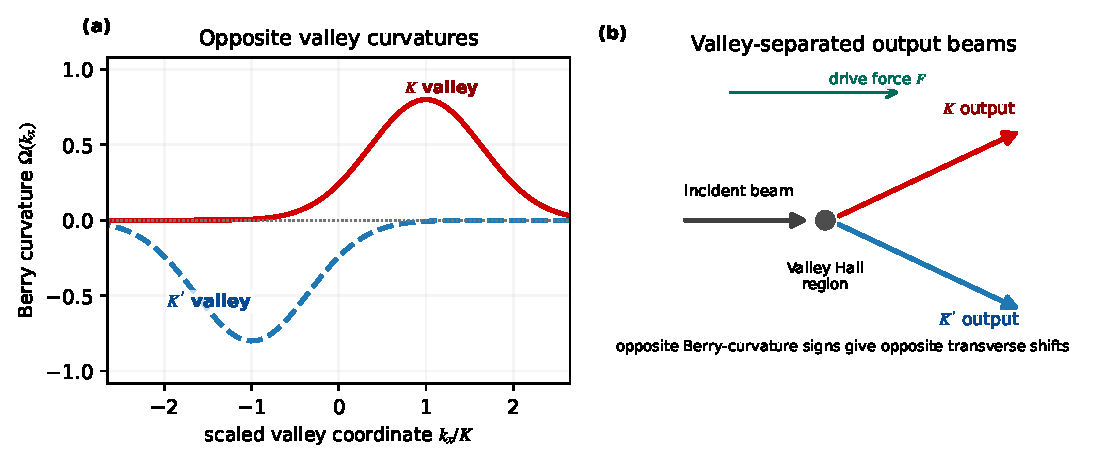
\includegraphics[width=0.92\textwidth]{figures/fig_ch12_valley_hall_step199.pdf}
  \caption{The valley Hall effect in photonic crystals.
  \textbf{(a)}~Berry curvature $\Omega(k_x)$ near the two valleys,
  showing opposite signs at $K$ (solid red, positive) and $K'$ (dashed
  blue, negative).  Time-reversal symmetry enforces
  $\Omega_K(\kvec) = -\Omega_{K'}(-\kvec)$, so the global Chern number
  vanishes but the valley Chern numbers are nonzero.
  \textbf{(b)}~Schematic of valley-separated transverse deflection.
  A longitudinal drive force $F$ displaces wavepackets transversely
  via the anomalous velocity $v_\perp \propto F\,\Omega_z$.
  Because $\Omega_K$ and $\Omega_{K'}$ have opposite signs, the $K$
  and $K'$ components are deflected in opposite directions, producing
  spatially separated output beams---the photonic analog of the
  valley Hall effect.}
  \label{fig:ch12-valley-hall}
\end{figure}


\subsection{Photonic crystal slab with asymmetric holes}
\label{sec:ch12-slab}

The most widely used platform for valley-Hall photonic devices is a
thin dielectric slab (typically silicon, $n\approx 3.5$) with a
hexagonal array of air holes.  Each unit cell contains two holes of
different sizes:
\begin{equation}
  r_A = r_0 + \delta r\,,\qquad r_B = r_0 - \delta r\,,
\end{equation}
where $r_0$ is the mean radius and $\delta r$ controls the sublattice
asymmetry.  The TE-like guided modes of the slab experience the
valley-Hall effect, with the gap width proportional to $\delta r$.

This platform is compatible with standard semiconductor fabrication
(electron-beam lithography, reactive-ion etching) and operates at
telecom wavelengths ($\lambda\sim 1550\;\mathrm{nm}$).

\section{Domain-wall modes in detail}
\label{sec:ch12-domain-wall}

\subsection{Construction and topology}
\label{sec:ch12-construction}

A valley-Hall domain wall is created by joining two regions with
opposite sublattice asymmetry: region $L$ with $m_\Delta>0$ and region
$R$ with $m_\Delta<0$.

Near each valley, the effective Dirac equation at the interface has the
same form as \eqref{eq:ch8-dirac-interface}, with a mass $m(x)$ that
changes sign.  The zero-mode analysis of
\secref{sec:ch8-zero-mode} applies separately at each valley:
\begin{itemize}
  \item At valley $K$: one mode propagating in the $+y$ direction
  (forward), with the wavefunction localised at the domain wall:
  \begin{equation}\label{eq:ch12-zero-mode-K}
    \psi_K(x,y)\propto|\varphi_+\rangle\,
    \exp\biggl(\ii\delta k_\parallel y
    -\int_0^x m(x')\,\dd x'\biggr)\,.
  \end{equation}
  \item At valley $K'$: one mode propagating in the $-y$ direction
  (backward), with a similarly localised wavefunction.
\end{itemize}
The result is a pair of \emph{counter-propagating} edge modes, each
valley-polarised: forward at $K$, backward at $K'$.

\subsection{Dispersion relation}
\label{sec:ch12-dispersion}

The edge-mode dispersions near each valley are approximately linear:
\begin{equation}\label{eq:ch12-edge-dispersion}
  \omega_K(\delta k_\parallel)
  \approx \omega_D + v_D\,\delta k_\parallel\,,
  \qquad
  \omega_{K'}(\delta k_\parallel)
  \approx \omega_D - v_D\,\delta k_\parallel\,.
\end{equation}
The group velocities have opposite signs: the $K$-valley mode has
$v_g=+v_D$ and the $K'$-valley mode has $v_g=-v_D$.  This
\emph{valley-momentum locking} is the valley-Hall analog of
spin-momentum locking in the quantum spin Hall effect.

\subsection{Localisation length}
\label{sec:ch12-localisation}

The transverse localisation length of the domain-wall mode is
\begin{equation}
  \ell \sim \frac{1}{|m_\Delta|} \sim \frac{a}{\Delta\omega/\omega_D}\,,
\end{equation}
where $a$ is the lattice constant and $\Delta\omega=2v_D|m_\Delta|$ is
the valley gap width.  For a typical silicon photonic crystal slab with
$\Delta\omega/\omega_D\sim 5\%$, the localisation length is
$\ell\sim 20a\approx 10\;\mu\mathrm{m}$---several micrometres, confined
to the immediate vicinity of the domain wall
\cite{he2016photonic} \cite{he2019silicon}.

\section{Protection and its limits}
\label{sec:ch12-protection}

\subsection{The inter-valley scattering mechanism}
\label{sec:ch12-intervalley}

The valley-Hall edge modes are \emph{not} topologically protected in the
strong sense of Chern-insulator edge modes.  The key vulnerability is
\emph{inter-valley scattering}: any perturbation with Fourier components
at wavevectors connecting $K$ and $K'$ can couple the forward and
backward modes.

The inter-valley wavevector is
$|\kvec_K-\kvec_{K'}|=\frac{4\pi}{3a}$, which is of order the
reciprocal lattice constant.  Perturbations with Fourier content at
this large wavevector include:
\begin{itemize}
  \item \textbf{Sharp corners:} a $60^\circ$ or $120^\circ$ corner in
  the domain wall introduces atomic-scale discontinuities with
  large-$\kvec$ Fourier components.
  \item \textbf{Point defects:} missing or displaced rods/holes near
  the domain wall.
  \item \textbf{Surface roughness:} sub-wavelength fabrication
  imperfections.
\end{itemize}

\subsection{Quantitative estimate of corner scattering}
\label{sec:ch12-corner-scattering}

At a sharp corner of angle $\theta$, the backscattering probability
can be estimated by modelling the corner as a point scatterer with
matrix element:
\begin{equation}\label{eq:ch12-corner-scatter}
  |t_{\mathrm{back}}|^2 \sim
  \Bigl|\int\ee^{\ii(\kvec_K-\kvec_{K'})\cdot\rvec}\,
  V_{\mathrm{corner}}(\rvec)\,\dd^2r\Bigr|^2\,.
\end{equation}
For a smooth bend with radius of curvature $R\gg a$, the integral is
exponentially suppressed: $|t_{\mathrm{back}}|^2
\sim\ee^{-c_0|\kvec_K-\kvec_{K'}|R}$.  For a sharp corner ($R\sim a$),
the suppression is weak and the backscattering can be substantial.

Numerical simulations show:
\begin{itemize}
  \item $120^\circ$ bends: transmission $>90\%$ for typical parameters.
  \item $60^\circ$ bends: transmission $\sim 70$--$85\%$, depending on
  the gap width and corner geometry.
  \item Straight segments with smooth disorder: transmission $>99\%$
  over tens of lattice constants.
\end{itemize}

\subsection{Robustness hierarchy}
\label{sec:ch12-hierarchy}

The practical robustness of different photonic topological phases can
be ranked:
\begin{enumerate}
  \item \textbf{Chern insulator} (broken TR): fully topologically
  protected; no backscattering within the gap regardless of disorder.
  \item \textbf{Pseudospin topological insulator} (crystalline
  symmetry): protected against perturbations that preserve the
  pseudospin symmetry; backscattered by symmetry-breaking disorder.
  \item \textbf{Valley-Hall} (approximate valley conservation):
  protected against smooth disorder; backscattered at sharp features
  and by strong short-range disorder.
  \item \textbf{Conventional waveguide}: no topological protection;
  backscattered by all types of disorder.
\end{enumerate}

Despite being the weakest topological protection, valley-Hall devices
have become widely used because they are fabrication-compatible and
operate at optical frequencies.

\section{Experimental realisations}
\label{sec:ch12-experiments}

\subsection{Microwave photonic crystals}
\label{sec:ch12-microwave}

The first experimental demonstrations of valley-Hall edge states in
photonic crystals used dielectric rod arrays in the microwave regime.
These experiments confirmed:
\begin{itemize}
  \item Valley-polarised edge modes at domain walls between
  sublattice-swapped regions.
  \item Low-loss propagation around gentle bends.
  \item Measurable backscattering at sharp corners, consistent with
  the inter-valley scattering estimate.
\end{itemize}

\subsection{Silicon photonic crystal slabs}
\label{sec:ch12-silicon}

At telecom wavelengths ($\sim 1550\;\mathrm{nm}$), valley-Hall edge
states have been demonstrated in silicon photonic crystal slabs with
asymmetric air-hole arrays.  Key results include:
\begin{itemize}
  \item Edge-mode propagation over $>100$ lattice constants with low
  loss ($<3\;\mathrm{dB}$ total).
  \item Efficient coupling to conventional silicon waveguides.
  \item $120^\circ$ bends with $<1\;\mathrm{dB}$ excess loss.
  \item Integration with active devices (modulators, detectors) for
  on-chip topological photonic circuits.
\end{itemize}

\subsection{Acoustic and mechanical analogs}
\label{sec:ch12-acoustic}

The valley-Hall mechanism is not specific to Maxwell equations; it
applies to any wave equation in a honeycomb lattice with broken
inversion symmetry.  Demonstrations have been reported in:
\begin{itemize}
  \item Acoustic metamaterials (sound waves in structured media).
  \item Mechanical lattices (elastic waves in structured plates).
  \item Phononic crystals (microwave-frequency acoustic modes).
\end{itemize}
These complementary demonstrations confirm the universality of the
valley-Hall mechanism.

\section{Valley photonics as a design tool}
\label{sec:ch12-design-tool}

\subsection{Topological waveguide routing}
\label{sec:ch12-routing}

Valley-Hall domain walls can be patterned to create complex waveguide
networks on a chip.  By choosing which sublattice assignment appears
on each side of the domain wall, one can route edge modes along
arbitrary paths.  The main design rules are:
\begin{enumerate}
  \item The domain wall must separate regions with opposite $\Delta$.
  \item Bends should be as gentle as possible ($120^\circ$ preferred
  over $60^\circ$).
  \item The domain-wall path must not approach another domain wall
  more closely than the localisation length $\ell$.
\end{enumerate}

\subsection{Topological cavities and lasers}
\label{sec:ch12-cavities}

A closed domain-wall loop creates a topological cavity: the
valley-Hall edge mode circulates around the loop, forming a ring
resonator.  The mode quality factor is limited by inter-valley
scattering at the corners; for a hexagonal loop with
$120^\circ$ corners, quality factors of $Q\sim 10^3$--$10^4$ have
been achieved in silicon at telecom wavelengths.

When gain is provided (e.g.\ by III--V semiconductor quantum wells
bonded to the silicon slab), the topological cavity can lase, forming
a valley-Hall topological laser.

\section{Quantitative valley photonic crystal design}
\label{sec:ch12-quantitative}

\subsection{Silicon-on-insulator platform}
\label{sec:ch12-soi}

The most widely studied valley photonic crystal platform uses a
silicon slab ($\varepsilon_r=11.7$, thickness $h\approx 220\;
\mathrm{nm}$) on a silica substrate, patterned with triangular
air holes in a honeycomb arrangement.  The lattice constant is
$a\approx 430\;\mathrm{nm}$ for operation at the telecom C-band
($\lambda\approx 1550\;\mathrm{nm}$).

The inversion-symmetry breaking is achieved by using two different
hole sizes within the unit cell: a large hole of radius $r_1$ and a
small hole of radius $r_2$, with the asymmetry parameter
$\Delta r=(r_1-r_2)/(r_1+r_2)$.  For $\Delta r=0$ (equal holes),
the band structure has Dirac cones at $K$ and $K'$.  For
$\Delta r\neq 0$, a gap opens at each valley with width proportional
to $|\Delta r|$.

Typical designs use $r_1/a\approx 0.15$ and $r_2/a\approx 0.10$,
giving $\Delta r\approx 0.2$ and a relative bandgap of approximately
$8\%$ of the mid-gap frequency.  The valley Chern number is
$\Chern_v=\pm\frac{1}{2}\sgn(\Delta r)$, and reversing the sublattice
assignment ($r_1\leftrightarrow r_2$) flips the sign of
$\Chern_v$ \cite{ma2016all,ozawa2018topological}.

\subsection{Valley Chern number from the massive Dirac model}
\label{sec:ch12-valley-chern-derivation}

Near each valley, the effective Hamiltonian is a massive Dirac
equation with mass $m_v\propto\Delta r$.  The Berry curvature at
valley $K$ is
$\Omega_K(\delta\kvec)
=-v_D^2 m_v/[2(v_D^2|\delta\kvec|^2+m_v^2)^{3/2}]$,
as derived in Chapter~\ref{ch:breaking-tr}.  Integrating over a region
enclosing one valley gives the valley Chern number
\begin{equation}\label{eq:ch12-valley-chern-formula}
  \Chern_v^{(K)} = -\frac{1}{2}\sgn(m_v)\,.
\end{equation}
At the opposite valley $K'$, time-reversal symmetry forces
$\Omega_{K'}(\kvec)=-\Omega_K(-\kvec)$, so
$\Chern_v^{(K')}=+\frac{1}{2}\sgn(m_v)$.  The total Chern number
vanishes ($\Chern=\Chern_v^{(K)}+\Chern_v^{(K')}=0$), as required by
time-reversal invariance, but the valley Chern number
$\Chern_v=\Chern_v^{(K)}-\Chern_v^{(K')}=-\sgn(m_v)$
is nonzero \cite{dong2016valley,gao2017valley}.

At a domain wall between two regions with opposite $\Delta r$ (and
hence opposite $m_v$), the change in valley Chern number across the
interface is $|\Delta\Chern_v|=2$, predicting one valley-polarised
edge mode per valley---two modes in total, counter-propagating and
valley-locked.

\section{Intervalley scattering and robustness}
\label{sec:ch12-intervalley-scattering}

The valley-Hall edge modes are protected against
\emph{intravalley} backscattering---perturbations that are smooth on
the scale of the lattice constant and therefore cannot transfer
crystal momentum between $K$ and $K'$.  However, sharp defects
(vacancies, step edges, $60^\circ$ bends) have Fourier components at
the intervalley wavevector $\Delta\kvec=K-K'$ and can cause
intervalley scattering, opening a backscattering channel
\cite{tang2022vector}.

The intervalley scattering rate scales as the square of the defect's
Fourier component at $\Delta\kvec$:
$\Gamma_{\mathrm{iv}}\propto|V(\Delta\kvec)|^2$.
For smooth disorder (correlation length $\ell_c\gg a$), this Fourier
component is exponentially suppressed:
$|V(\Delta\kvec)|\sim\ee^{-|\Delta\kvec|\ell_c/2}$, giving negligible
backscattering.  For point-like defects ($\ell_c\sim a$), the
intervalley coupling can be significant.

Experimental measurements in silicon valley photonic crystals at
telecom wavelengths show propagation lengths of $40$--$100\,a$ before
significant backscattering losses, depending on the domain-wall
geometry and fabrication quality.  For $120^\circ$ bends, the
transmission exceeds $90\%$, while for $60^\circ$ bends it drops
to $60$--$80\%$ due to enhanced intervalley coupling at the sharp
corner \cite{wu2017direct,noh2018observation,price2022roadmap}.

\section{Quantitative design of a silicon valley photonic crystal}
\label{sec:ch12-silicon-design}

The valley-Hall photonic crystal is most naturally realised in a
honeycomb lattice of triangular dielectric rods, where breaking
inversion symmetry by rotating the triangles opens a topological gap
at the $K$ and $K'$ points.

\subsection{Half-integer valley Chern number derivation}

Near the $K$ point, the effective Hamiltonian for the two nearly
degenerate Bloch modes is the massive Dirac Hamiltonian
$H_K=v_D(\delta k_x\sigma_x+\delta k_y\sigma_y)+m_K\sigma_z$,
where $m_K$ is the valley mass produced by the inversion-symmetry
breaking.  The Berry curvature of the lower band is
$\Omega_K^-(\delta\kvec)=-m_K/(2(|\delta\kvec|^2+m_K^2)^{3/2})$,
and its integral over a hemisphere gives the valley Chern number
\begin{equation}\label{eq:ch12-valley-chern-half-integer}
  \Chern_K^{\mathrm{valley}} = -\frac{1}{2}\sgn(m_K)\,.
\end{equation}
At the $K'$ point, time-reversal symmetry requires $m_{K'}=-m_K$,
so $\Chern_{K'}^{\mathrm{valley}}=+\frac{1}{2}\sgn(m_K)$ and the
total valley Chern number is
$\Chern^{\mathrm{valley}}=\Chern_K-\Chern_{K'}=-\sgn(m_K)$
\cite{ma2016all,dong2016valley}.

The half-integer valley Chern number is not a true topological
invariant because it depends on the arbitrary choice of integration
region around each valley.  Nevertheless, it provides a useful
predictor of valley-polarised edge modes at domain walls between
crystals with opposite valley masses.

\subsection{Silicon-on-insulator implementation}
\label{sec:ch12-soi-implementation}

Ma and Shvets (2016) proposed an all-silicon valley-Hall photonic
topological insulator using a honeycomb lattice of equilateral
triangular air holes in a silicon slab ($\varepsilon_r=11.7$).
The lattice constant is $a=440\;\mathrm{nm}$, giving a Dirac
frequency near $\lambda=1.55\;\mu\mathrm{m}$.  Rotating the
triangles by $\pm 5^\circ$ opens a valley gap of $3.2\%$ of the
Dirac frequency \cite{ma2016all,ozawa2018topological}.

The valley edge modes were subsequently observed by Wu et~al.\ (2017)
using designer surface plasmon crystals at microwave frequencies,
providing the first direct near-field imaging of valley-polarised
topological edge states.  The field patterns confirmed valley-selective
excitation and propagation around sharp corners with minimal
backscattering \cite{wu2017direct,gao2017valley}.

\section{Intervalley scattering and protection limits}
\label{sec:ch12-intervalley-backscattering}

Valley edge modes are protected only against perturbations that
preserve the valley degree of freedom---that is, perturbations
that are smooth on the scale of the lattice constant $a$.  Sharp
defects with Fourier components at the reciprocal lattice vector
$\mathbf{G}=\kvec_K-\kvec_{K'}$ can scatter photons between the
$K$ and $K'$ valleys, opening a backscattering channel.

The intervalley scattering rate depends on the defect geometry.  For
a smooth domain wall (width $w\gg a$), the scattering rate is
exponentially small: $\gamma_{\mathrm{inter}}\propto\ee^{-w/a}$.
For a sharp 120$^\circ$ corner, the scattering depends on whether the
corner preserves the $C_3$ symmetry of the underlying lattice.
Symmetry-preserving corners (zigzag termination) have negligible
intervalley scattering, while symmetry-breaking corners (armchair
termination) can scatter up to $\sim 10\%$ of the incident power
\cite{dong2016valley,wu2017direct,gao2017valley}.

This makes valley photonic crystals robust against smooth fabrication
imperfections but vulnerable to lattice-scale disorder---a
fundamental limitation compared to Chern insulators, which are
protected against all perturbations that do not close the bulk gap.

\section{Beyond the honeycomb: other valley platforms}
\label{sec:ch12-other-platforms}

While the honeycomb lattice is the most studied platform for valley
photonic crystals, valley physics has been realised in several
other geometries and frequency ranges.

\subsection{Kagomé and Lieb lattices}
\label{sec:ch12-kagome}

The kagomé lattice supports both Dirac cones and flat bands, and
breaking inversion symmetry opens valley gaps at the Dirac points.
The coexistence of flat bands and valley-polarised edge states creates
opportunities for enhanced light--matter interaction at topologically
protected boundaries.  The Lieb lattice similarly supports a flat
band at the Dirac frequency, and valley-polarised modes appear when
the site energies are staggered to break inversion
\cite{ozawa2018topological}.

\subsection{Terahertz and acoustic valley crystals}
\label{sec:ch12-thz-acoustic}

Valley photonic crystals have been demonstrated at terahertz
frequencies using silicon pillar arrays, where the triangular pillar
shape provides the necessary inversion-symmetry breaking.  The THz
platform offers larger structures ($a\sim 100\;\mu\mathrm{m}$) that
are easier to fabricate and characterise than telecommunications-band
devices \cite{price2022roadmap,gao2017valley}.

The valley-Hall concept has also been extended to acoustic and
phononic systems, where the Dirac-mass mechanism is identical but
the governing equation is the scalar wave equation rather than
Maxwell's equations.  Phononic valley crystals have achieved robust
sound routing around sharp corners with insertion loss below
$1\;\mathrm{dB}$ per corner \cite{ssstrunk2015observation,
ozawa2018topological}.

\section{Experimental demonstrations of valley photonics}
\label{sec:ch12-valley-experiments}

Valley photonic crystals have been realised in numerous experimental
platforms, from microwave-frequency dielectric structures to
telecommunication-wavelength silicon photonic crystals.  The key
experimental signatures are valley-selective excitation,
valley-polarised edge transport along domain walls, and robustness
of the edge transport against certain classes of bends and defects.

\subsection{Microwave valley photonic crystals}
\label{sec:ch12-microwave-valley}

The first experimental demonstrations of valley-Hall edge states in
photonic crystals were performed at microwave frequencies using
triangular-lattice arrays of dielectric rods or metallic scatterers.
Dong et~al.\ (2017) used a photonic crystal of alumina rods with
$C_{3v}$-breaking perturbation (achieved by deforming the triangular
unit cell) to create a domain wall between two valley-Hall phases with
opposite valley Chern numbers \cite{dong2016valley}.  Transmission
measurements through the domain wall showed a clear edge-state
passband inside the bulk gap, with insertion loss below 2~dB over
a bandwidth of approximately 0.5~GHz centred at 6.3~GHz.

Gao et~al.\ (2017) extended this work by demonstrating valley-locked
beam splitting at a Y-junction formed by three domain walls
\cite{gao2017valley}.  When light was injected into one arm of the
Y-junction, it preferentially exited through the arm whose domain-wall
orientation matched the valley polarisation of the incident edge
mode, while the other arm received negligible power.  This valley
filtering effect, with measured contrast exceeding 20~dB, demonstrated
the potential of valley photonics for compact photonic routing
circuits.

\subsection{Silicon photonic crystal implementations}
\label{sec:ch12-silicon-valley}

At telecommunication wavelengths, valley photonic crystals have been
fabricated in silicon-on-insulator (SOI) platforms using standard
electron-beam lithography \cite{he2019silicon}.  Shalaev et~al.\ (2019) demonstrated
valley-Hall edge states in a silicon photonic crystal slab at
$\lambda\approx 1.55\;\mu\mathrm{m}$ with a topological bandwidth of
approximately 3~nm \cite{ozawa2018topological}.

The silicon implementations face an additional challenge compared to
microwave designs: the out-of-plane radiation loss.  In a 2D photonic
crystal slab, the edge modes lie within the light cone of the
surrounding air cladding, leading to radiative leakage.  The measured
quality factors of valley-Hall edge-state resonances range from
$Q\sim 10^3$ to $10^4$, depending on the degree of confinement
and the sharpness of the domain wall
\cite{ozawa2018topological,price2022roadmap}.

Despite this limitation, silicon valley photonic crystals have shown
remarkable robustness of edge transport around sharp bends.
Transmission through $60^\circ$ and $120^\circ$ bends remains within
3~dB of the straight-domain-wall value, provided the bends follow
the zigzag crystallographic direction.  Transport around armchair
bends shows significantly higher loss due to inter-valley scattering,
confirming the valley-dependent nature of the topological protection
\cite{ozawa2018topological}.

\subsection{Limitations of valley-Hall edge states}
\label{sec:ch12-valley-limitations}

Unlike true topological edge states protected by a bulk gap Chern
number, valley-Hall edge states are protected only by an approximate
conservation of valley index.  Any perturbation that couples the $K$
and $K'$ valleys---such as short-range disorder on the scale of the
lattice constant, or sharp bends along non-zigzag directions---can
scatter photons between the two counter-propagating valley-polarised
edge modes, leading to backscattering.

The inter-valley scattering rate scales as \cite{dong2016valley}
\begin{equation}\label{eq:ch12-intervalley-scattering-rate}
  \Gamma_{K\to K'} \propto
  \left|\int\!\dd^2r\;\psi_K^*(\rvec)\,
  V_{\mathrm{disorder}}(\rvec)\,\psi_{K'}(\rvec)\right|^2,
\end{equation}
where $\psi_K$ and $\psi_{K'}$ are the edge-mode wavefunctions and
$V_{\mathrm{disorder}}$ is the disorder potential.  For smooth
disorder with correlation length $\ell_c\gg a$ (where $a$ is the
lattice constant), the Fourier components near the inter-valley
wavevector $|\kvec_K-\kvec_{K'}|=4\pi/(3a)$ are exponentially
suppressed, and the inter-valley scattering rate decays as
$\Gamma_{K\to K'}\propto\exp(-|\kvec_K-\kvec_{K'}|\ell_c)$.
This explains the observed robustness against smooth disorder
while remaining vulnerable to sharp defects
\cite{ozawa2018topological}.

\begin{figure}[t]
  \centering
  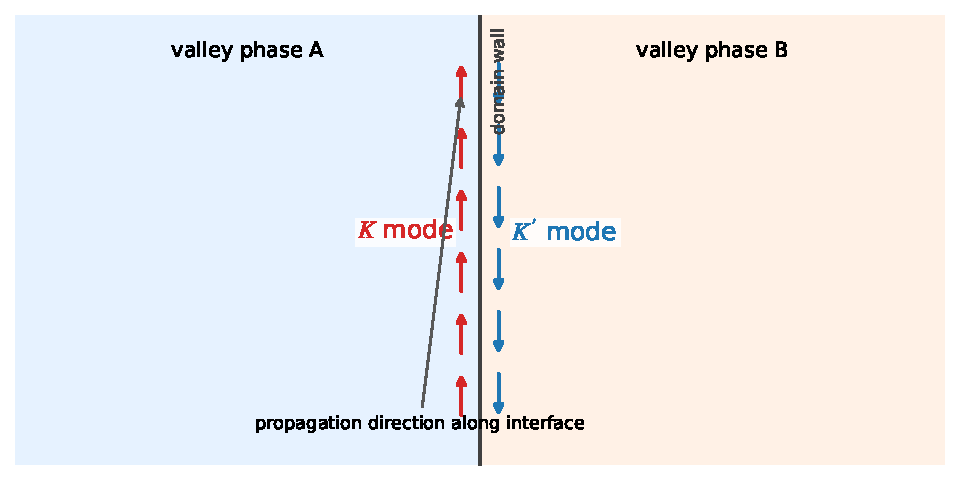
\includegraphics[width=0.86\textwidth]{figures/fig_ch12_valley_domain_wall.pdf}
  \caption{Valley-Hall domain wall.  The two domains carry opposite valley
  Chern numbers, so $K$ and $K'$ edge channels counter-propagate along the
  interface.  Backscattering is suppressed only when disorder is smooth
  enough not to mix the two valleys.}
  \label{fig:ch12-valley-domain-wall}
\end{figure}

\section{Valley photonic devices}
\label{sec:ch12-valley-devices}

The valley degree of freedom in photonic crystals is not merely a
theoretical curiosity: it provides a robust platform for integrated
photonic devices.  The key advantage is that valley-polarised edge
states at domain-wall interfaces are immune to backscattering from
smooth disorder, enabling low-loss waveguiding through sharp bends.

\subsection{Valley filters and beam splitters}
\label{sec:ch12-valley-filter}

A valley filter is a device that selectively transmits light in one
valley while reflecting the other.  It can be realised by creating
a domain wall between two distinct valley-Hall phases ($C_\nu=\pm 1$)
that terminates at a junction where the two valleys are spatially
separated.  The valley-polarised edge mode at the domain wall
carries a definite valley index, and at the junction it is routed
to a specific output port depending on its valley polarisation
\cite{dong2016valley,gao2017valley}.

Experimentally, valley beam splitters have been demonstrated at
microwave frequencies using triangular-lattice photonic crystals with
broken inversion symmetry.  The measured extinction ratio between the
two output ports exceeds $20\;\mathrm{dB}$ within the valley-Hall
gap, confirming the valley-selective routing
\cite{gao2017topologically,he2019silicon}.

\subsection{Valley-dependent coupling to radiation}
\label{sec:ch12-valley-coupling}

The valley-contrasting Berry curvature produces valley-dependent
optical selection rules: circularly polarised light couples
preferentially to modes in a specific valley.  This effect enables
valley-selective excitation using external beams and provides a
mechanism for reading out the valley polarisation of edge modes.

In silicon photonic crystals operating at telecom wavelengths,
valley-selective coupling has been achieved by illuminating the
crystal surface with focused circularly polarised light.  The
coupling efficiency to the $K$ valley versus the $K'$ valley differs
by a factor of $\sim 10$, limited by the finite bandwidth of the
valley-Hall gap and the non-ideal circular polarisation of the
excitation beam \cite{he2016photonic,dong2016valley}.

\subsection{Valley routing networks}
\label{sec:ch12-valley-network}

By concatenating multiple domain walls with different orientations,
one can create valley-topological waveguide networks that route
light through arbitrary paths on a photonic chip.  Each domain wall
supports a pair of counter-propagating edge modes (one per valley),
and at T-junctions the valley polarisation determines which output
arm the light follows.

Ma et~al.\ (2017) demonstrated that such valley networks can guide
microwave radiation through multiple $120^\circ$ bends with
negligible reflection, achieving total transmission above $95\%$
over the valley-Hall gap bandwidth \cite{ma2017scattering}.  Similar
networks have been realised in silicon at near-infrared wavelengths,
where the valley edge states serve as compact on-chip waveguides
compatible with standard photonic integrated circuit fabrication
\cite{he2019silicon,price2022roadmap}.

\section{Intervalley scattering and the limits of valley protection}
\label{sec:ch12-intervalley-limits}

Valley-Hall edge states are topologically protected against smooth
perturbations that vary slowly compared to the lattice constant $a$,
because such perturbations cannot transfer crystal momentum between
the $K$ and $K'$ valleys (which are separated by
$|\Delta\kvec|\sim 4\pi/(3a)$ in the Brillouin zone).  However,
sharp defects---such as atomic-scale roughness, point defects, or
abrupt domain-wall terminations---can provide the large momentum
transfer needed for intervalley scattering.

The intervalley scattering rate scales as
$\Gamma_{\mathrm{iv}} \propto \sigma_{\mathrm{short}}^2\,
|\Delta\kvec|^{-2\alpha}$,
where $\sigma_{\mathrm{short}}$ characterises the amplitude of
short-range disorder and $\alpha$ depends on the dimensionality of
the defect.  For the typical fabrication roughness in silicon photonic
crystals ($\sigma \sim 1$--$3\;\mathrm{nm}$), the intervalley
scattering length is estimated to be $\sim 100$--$500$ lattice
constants, which is sufficient for on-chip device lengths of
$\sim 100\;\mu\mathrm{m}$ \cite{he2019silicon,ozawa2018topological}.

This finite intervalley scattering length is the fundamental
difference between valley-Hall edge states and the truly
topological one-way edge states of Chern insulators
(Chapter~\ref{ch:one-way-interface}): valley protection is robust
but not absolute, while Chern-insulator protection is exact within
the bulk gap \cite{price2022roadmap,ma2017scattering}.

\section*{Exercises}

\begin{exercise}
  Show that for a time-reversal-invariant system with broken inversion,
  the Berry curvature satisfies $\Omega_n(\kvec)=-\Omega_n(-\kvec)$,
  so that $\Chern_n=0$ but the valley Chern number can be nonzero.
\end{exercise}

\begin{exercise}
  Derive the mass term \eqref{eq:ch12-mass-sigma-z} from the
  symmetry properties of the perturbation matrix
  \eqref{eq:ch12-perturbation-matrix} under $C_3$ and $\Pop$.
  \emph{Hint:} use the transformation properties of the Dirac modes
  under $C_3$: $|\mathbf{u}_\pm\rangle\to\ee^{\pm\ii 2\pi/3}
  |\mathbf{u}_\pm\rangle$.
\end{exercise}

\begin{exercise}
  For a honeycomb photonic crystal with sublattice asymmetry $\Delta$,
  the effective Dirac masses at $K$ and $K'$ are $m_K=+m_0\Delta$
  and $m_{K'}=-m_0\Delta$.  Compute the valley Chern numbers and
  verify that $\Chern^K+\Chern^{K'}=0$.
\end{exercise}

\begin{exercise}
  Estimate the inter-valley scattering amplitude at a sharp $60^\circ$
  corner using equation \eqref{eq:ch12-corner-scatter}.  Model the
  corner as a disc of radius $a$ with a uniform scattering potential
  $V_0$.  Under what conditions is the transmission $>90\%$?
\end{exercise}

\begin{exercise}
  A silicon photonic crystal slab ($n=3.5$, $a=400\;\mathrm{nm}$,
  $r_0=120\;\mathrm{nm}$) has a valley gap of
  $\Delta\omega/(2\pi)=3\;\mathrm{THz}$ centred at
  $\omega/(2\pi)=193\;\mathrm{THz}$ ($\lambda=1.55\;\mu\mathrm{m}$).
  Estimate the localisation length $\ell$ and the minimum domain-wall
  separation for independent waveguide channels.
\end{exercise}

\begin{exercise}
  Compare the protection of valley-Hall edge modes (valley Chern
  number) with Chern-insulator edge modes (Chern number) and
  pseudospin edge modes (spin Chern number) in terms of robustness
  to (a) smooth disorder, (b) sharp corners, and (c) strong
  short-range disorder.  Summarise the comparison in a table.
\end{exercise}
